\documentclass[11]{article}

\usepackage{graphicx}
\usepackage{url}
\usepackage{float}
\usepackage{caption}
\usepackage[margin = 1in]{geometry}
\usepackage{indentfirst}
\usepackage{natbib}
\usepackage{subcaption}

%underlines the title of a book/article in the References section (ideal for UWS Harvard style)
%FIXME check that all the citation rules are obeyed.
\usepackage{ulem}

\begin{document}

\title{ASP.NET vs PHP}
\author{Marius Olariu (B00350529)}
\date{}
\maketitle

\section{Introduction}(500 words)\\

\bibpunct{(}{)}{;}{a}{,}{}

	Nowadays, people expect personalized experiences and the Internet makes no exception to this rule. In order to fulfill this user requirement we need dynamic webpages (i.e. pages that can change automatically the content they display), few webpages currently are static (i.e. have the same content every time you open them). An example of a dynamic webpage could be \textit{amazon.com} that displays on the home page products that you might be interested in (based on your previous purchases, search history) whereas an example of a static webpage could be the contents of a book published online (e.g. https://natureofcode.com/book/). Developers automatically wonder what are the best technologies to use in order to develop dynamic webpages. However, due to the fact that different dynamic webpages have different requirements this study-case is going to focus on comparing two web technologies suitabale for developing a future version of \textit{www.uws.ac.uk}, namely ASP.NET and PHP. One of the main requirements of this site is to be able to process a lot of data (e.g. a lot of applications for programmes provided by university) thus it uses a SQL database sytem to store it. This study-case is going to compare how the aforementioned technologies interract with SQL database systems. \\ 
	
	ASP.NET is a framework from Microsoft for building dynamic web pages that was released in 2002 as a successor to \textbf{A}ctive \textbf{S}erver \textbf{P}ages (ASP).  This technology is used in the server-side web development; in other words, it interacts with the "computer" processing the website request and produces web pages that contain only HTML, CSS and JavaScript. ASP.NET provides flexibility to the developers because they have multiple choices when it comes to what languages to use for the backend of the website, namely ASP.NET supports C\#, Visual Basic .NET and J\# (a language inspired by Java). Additionally, writing the backend in C\# or J\# speeds the process of providing the website to the client because these languages are compiled (the backend code does not have to be interpreted at runtime). In 2014 Microsoft made the .NET server stack open-source (ASP.NET, .NET compiler, .NET Core Runtime etc.), ASP.NET can be found on a GitHub repository (\textit{github.com/aspnet}). Moreover, in the same year they started to support cross-platform development by making the tools needed available for platforms like Linux or macOS and deployment on a Linux web server.\\
	
	PHP is one of the most used programming languages \citep{cass2014top, cass20152015} and it is mainly used to write the backend of a webpage, in other words, mainly a server-side language . PHP was released in 1994 and the acronym stands for \textit{Hypertext Preprocessor}  or \textit{Personal Home Page Tools}, the later variant being the original name. The main advantage of this language is the fact that it can be embedded in HTML code and after being interpreted the PHP code results is HTML code (that gets sent to the browser). It is worth mentioning that PHP development is now open-source. Websites developed using PHP for the backend are cross-platform, namely, they can be hosted on web servers running Linux or Windows. The widely adoption of this language is due to the fact that is free and runs fast in combination with Apache and MySql on a low-specifications web server~\citep{converse2004php5}. Another reason for the use of PHP is that it is easy to learn.

\pagebreak

\section{Body}(2500 words)
%The body must present a comparison between ASP.NET and PHP web sites when used with typical SQL-based database management systems.
%In particular, you should present what you consider to be the five most important factors when comparing these two technologies.

	The above technologies are analysed based on how they interract with \textbf{R}elational \textbf{D}atabase \textbf{M}anagement \textbf{S}ystems (RDBMS). In order to manipulate the data stored in a RDBMS the standard language is \textbf{S}tructured \textbf{Q}uery \textbf{L}anguage (SQL) that is why these RDBMS are sometime referred as \textit{SQL-databases}. There are many RDBMS systems out there, to mention but a few: Oracle, MySQL, Microsoft SQL Server, PostgreSQL etc. . PHP websites use mostly MySQL because these two technologies have been developed with each other in mind, are both open source projects with active web communities around them and (as mentioned above) are fast~\citep{davis2007learning}. ASP.NET websites use mostly Microsoft SQL Server because both technologies are developed and maintained by Microsoft. 

%Given the above mentioned things about the bounds between the technologies, the first thing to analyze is how  these two technologies interract with MySql and SQL Server.\\ 

%	\subsection{MySQL}
%	First, let's have a look on how PHP is used with MySQL. PHP5 provides native APIs in order to connect to MySQL, namely \textit{mysql}, {mysqli}  and \textit{PDO\_MySQL}. However, starting with PHP7 the \textit{mysql} extension is deprecated.

%	Second, let's have a look on how ASP.NET is used with MS SQL Server. \\

%	Can you use PHP and MS SQL Server? What about ASP.NET and MySQL.

	\subsection{Storage}
		In the past database storage was quite expensive but as the hardware technology advances and new discoveries are put in practice, for example (if cloud storage is chosen) having data centers at the bottom of oceans~\citep{simon2018project}, the price of storage is becoming cheaper. Nonetheless, there are few things that have to be taken into account when choosing a database system. The considerations will be briefly mentioned and then there is going to be analyzed how the two programming technologies interract.

	\subsubsection{Scalability\\}
	As the university keeps expanding, for example - opens new campuses, it is likely that a type of SQL-database cannot keep the pace with the new requirements for \textit{uws.ac.uk} (e.g. store  retrieve more data) thus it would be wise to pick a database system that offers  easy migration of data to another database management system.

	\subsubsection{Database replication\\}
	No matter how scalabale a database is at some point the database needs to be replicated in more than one server. This creates the need of keeping the servers synched, thus there is created a \textit{master-slave} relationship between the database servers. Usually the inserts happen in the master database and the reads are supplied by the slave databases (they keep synched with the master database by periodically updating thei content). Moreover, in case the master database fails one of the slaves databases could take the place to ensure availability of the website.

	\subsubsection{GUI Interface \\}
	Often there is a need to interact directly with the database so a GUI can be really helpful, whether a web interface or a native software for a specific OS.\\

	PHP offers native support for the following types of databases.

		\begin{table}[H]
			\caption{Main databases supported by PHP through native APIs~\citep{PhpDbs}}
			  \centering
				\begin{tabular}{|l|l|l|}
					\hline
					\textbf{Name} & \textbf{Type} & \textbf{Language}\\
					\hline
					Cubrid & Relational & SQL\\
					\hline
					DB++ & Relational & AQl\\
					\hline
					dBase & Relational & dBase\\
					\hline
					InterBase & Relational & SQL\\
					\hline 
					FrontBase & Relational & SQL\\
					\hline 
					IBM Db2 & Relational & SQL\\
					\hline 
					IBM Informix & Relational & SQL\\
					\hline 
					Ingres & Relational & QUEL\\
					\hline 
					MaxDb & Relational & SQL\\
					\hline 
					MongoDB & Document-oriented database & Mongo Shell\\
					\hline 
					mSQL & Relational & SQL\\
					\hline 
					Microsoft SQL Server & Relational & SQL\\
					\hline 
					MySQL& Relational & SQL\\
					\hline 
					Oracle  & Relational & SQL\\
					\hline 
					PostgreSql  & Object-Relational & SQL\\
					\hline 
					Paradox  & Relational & PAL\\
					\hline 
					Ingres & Relational & QUEL\\
					\hline 
				\end{tabular}
		\end{table}

		ASP.NET developers can work with a database using \textbf{E}ntity \textbf{F}ramework \textbf{C}ore (EFC), a object-relational mapping that uses .NET objects to manipulate data. ASP.NET supports the following databases.

		\begin{table}[H]
			\caption{Main databases supported by ASP.NET through EFC~\citep{AspDbs}}
			  \centering
				\begin{tabular}{|l|l|l|}
					\hline
					\textbf{Name} & \textbf{Type} & \textbf{Language}\\
					\hline
					MariaDB & Relational & SQL\\
					\hline
					MyCAT Server& Relational & SQl\\
					\hline
					Firebird & Relational & SQL\\
					\hline 
					Progress OpenEdge & Relational & OpenEdge ABL\\
					\hline 
					IBM Db2 & Relational & SQL\\
					\hline 
					IBM Informix & Relational & SQL\\
					\hline 
					Ingres & Relational & QUEL\\
					\hline 
					Microsoft SQL Server & Relational & SQL\\
					\hline 
					MySQL& Relational & SQL\\
					\hline 
					Oracle  & Relational & SQL\\
					\hline 
					PostgreSql  & Object-Relational & SQL\\
					\hline 
				\end{tabular}

		\end{table}


	As can be seen above, for both technologies there is a large variety of databases available. Some databases are available for both technologies like Oracle, PostgreSql, MySQL, Microsoft SQL Server, Ingres, IBM Informix, IBM Db2. There can be said that PHP offers support for almost every database that ASP.NET supports and some more. Therefore, if one is looking for database scalability (see 2.1.1) it is better to develop the backend in PHP.\\
	\indent
	When it comes to GUI Interfaces (see 2.1.2.) most of them provide at least a web GUI. One could look further to see which type of database provides the best GUI or the largest number of GUIs (e.g. web, native application etc.) but this is beyond the purpose of this work. Again, it seems that PHP is more likely to be the right choice.\\

%talk about how php and asp.net connect to different dbs and how these satisfy the aforementioned useful db characteristics

%Windows OS on server is not free
%Sql server isn't free as well
	

	\subsection{Cost}
	The mass adoption of PHP was due to the fact that it was open-source and able to used in combination with free software like Apache, MySQL and Linux. By contrast, in order to develop dynamic webpages with ASP.NET you had to buy a licence for the IDE, pay for Microsoft SqL Server licence, host your wepage on a Windows web server and so on, however, all this changed when the development for ASP.NET went open-source, Visual Studio free and the deployment of webpage on a Linux web server was possible through the \cite{Mono}. This was a big and important step for Microsoft. Moreover, now the ASP.NET supports connection to free databases like MySQL. From what was stated above it can be said that the costs are pretty similar.\\
	\indent
	A future version of a webpage like \textit{uws.ac.uk} would need a team of developers in order to be developed professionally and according to \textit{payscale.com} the average salary for a PHP developer is less than the average salary for a ASP.NET developer. Therefore, if not for the cost of a certain stack of technologies used then at least from the perspective of workforce cost PHP is cheaper.

		\begin{figure}
				\centering
						\begin{subfigure}{.5\textwidth}
						  \centering
						  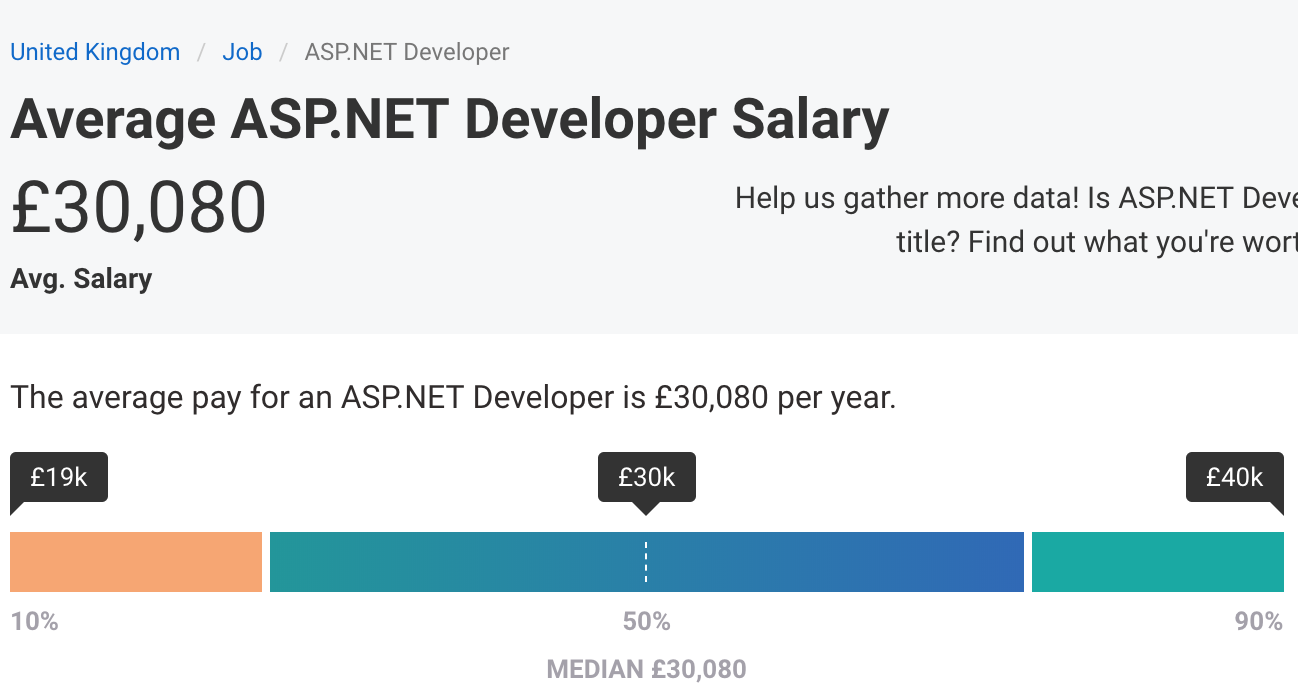
\includegraphics[scale=0.45]{aspSalary}
						  \caption{Average salary for a ASP.NET developer in UK}
						  \label{fig:sub1}
						\end{subfigure}%

						\begin{subfigure}{.5\textwidth}
						  \centering
						  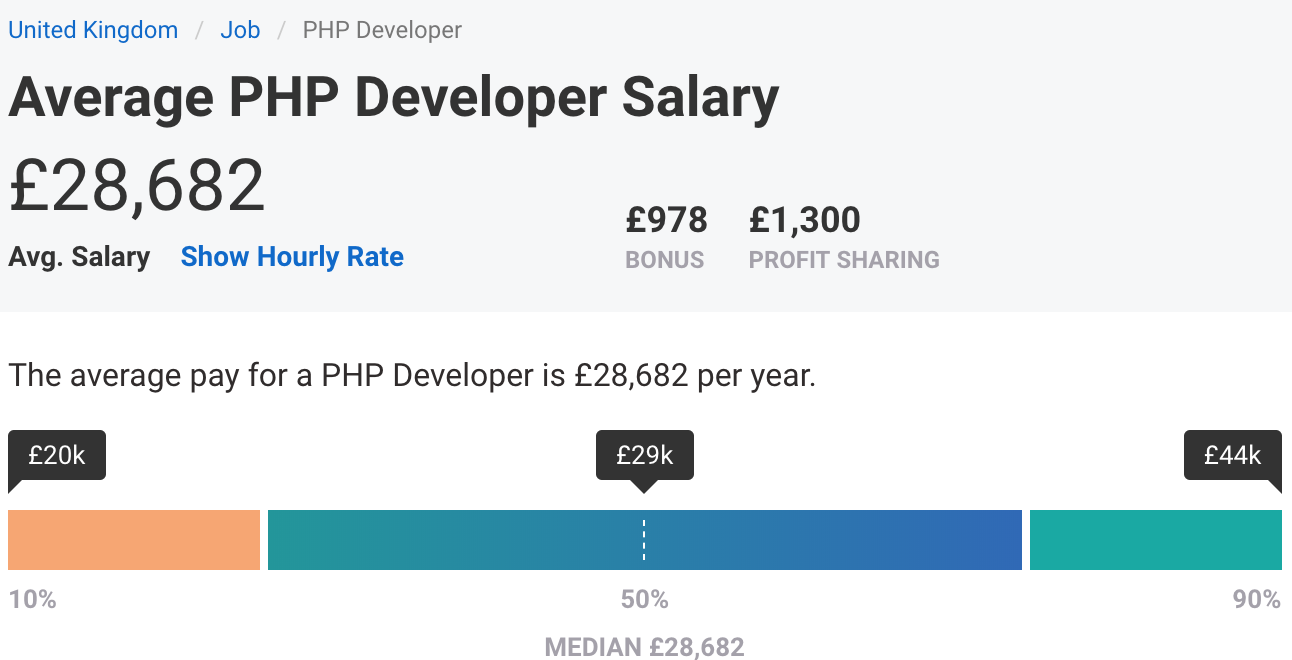
\includegraphics[scale=0.45]{phpSalary}
						  \caption{Average salary for a PHP developer in UK}
						  \label{fig:sub2}
						\end{subfigure}

				\caption{Comparison between salaries of PHP/ASP.NET developers}
				\label{salaryComp}
		\end{figure}
	
	\subsection{Security}

	\subsection{Maintenance available (or commercial license)}

	\subsection{Development}
	The technologies can be compared also by the underlying programming paradigm that they use. In the case of ASP.NET, because it is a framework, C\# will be the chosen language for comparison since it is the most popular choice from all of the possibilites. \\
	
	\indent
	PHP started as a scripting language in 1995, however, it has moved towards the Object Oriented paradigm supporting concepts like class, object, constructors \& destructors or object inheritance~\citep{PhpOop}. For a language to be considered Object-Oriented it needs to adhere to three main concepts: \textbf{Encapsulation}, \textbf{Polymorphism} and \textbf{Inheritance}. Encapsulation is used to bundle data and methods to a class, to protect the state of an object and it is achieved in PHP through the access specifies like \textit{public}, \textit{private} and \textit{protected}. Polymorphism is the ability to provide a interface to entities of different types and it is achieved in PHP by having \textit{interfaces} and \textit{abstract classes}. Inheritance allows new objects to "inherit" the properties and services of existing objects and is achieved in PHP by allowing classes to be \textit{extended} and interfaces to be \textit{implemented}. To sum it up, PHP7 can be considered an Object Oriented language but there some problems due to the fact that it has to be compatible with legacy code and the fact that it was not designed from the start as an Object Oriented language.\\
	By comparison, C\# is a robust and mature Object Oriented language and it allows the programmer to develop good designed software that promotes separation of content, logic and data and thus the software it is easier to support in the long run. In addition, ASP.NET provides well-organized libraries that allow the developer to create new features easily  whereas in PHP it might be slightly harder to develop the same funcionality by using libraries developed by different developers. \\

	\indent
	A big part of the development time is spent on debugging the code and  testing it. PHP does not offer great tools for debugging, often, the developer has to use third-party software. ASP.NET provides free of charge an Integrated Development Environment (IDE) for computers running Windows/macOS which allows debugging of webpages code.\\
	
	\indent
	In the first versions of PHP there was no mechanism for error traping but this drawback was fixed in PHP5 when \textit{Exception Handling} was added. Thus, from this way of looking at it, PHP5 is similar to C\#.\\
	
	\indent
	Taking into account the strictly the development part it seems that ASP.NET would be a better choice for \textit{uws.ac.uk}.  


	\subsection{Speed}
%alexa.com info
%sumarise the webpage load speed
   According to \textit{similartech.com}, a website which performs comparisons between technologies, ASP.NET was used in the development of about 2.5 million websites whereas PHP was used for the developemnt of about 7.5 million websites~\citep{CompPhpAsp}~\ref{websites}. These numbers suggests that both of them are valid technologies used by industry. One way to compare the two technologies would be by the webpage load speed. As can be found on Alexa's website, a company owned by Amazon, the current version of \textit{uws.ac.uk} loads pretty slow, on average 3.64 seconds and 83\% of websites load faster~\citep{LoadSpeed}.
It is generally believed that  ASP.NET is faster than PHP because it can use for the backend programming languages that are compiled, like C\#, whereas PHP is an interpreted language. \\

	\begin{figure}[H]

			\begin{center}
					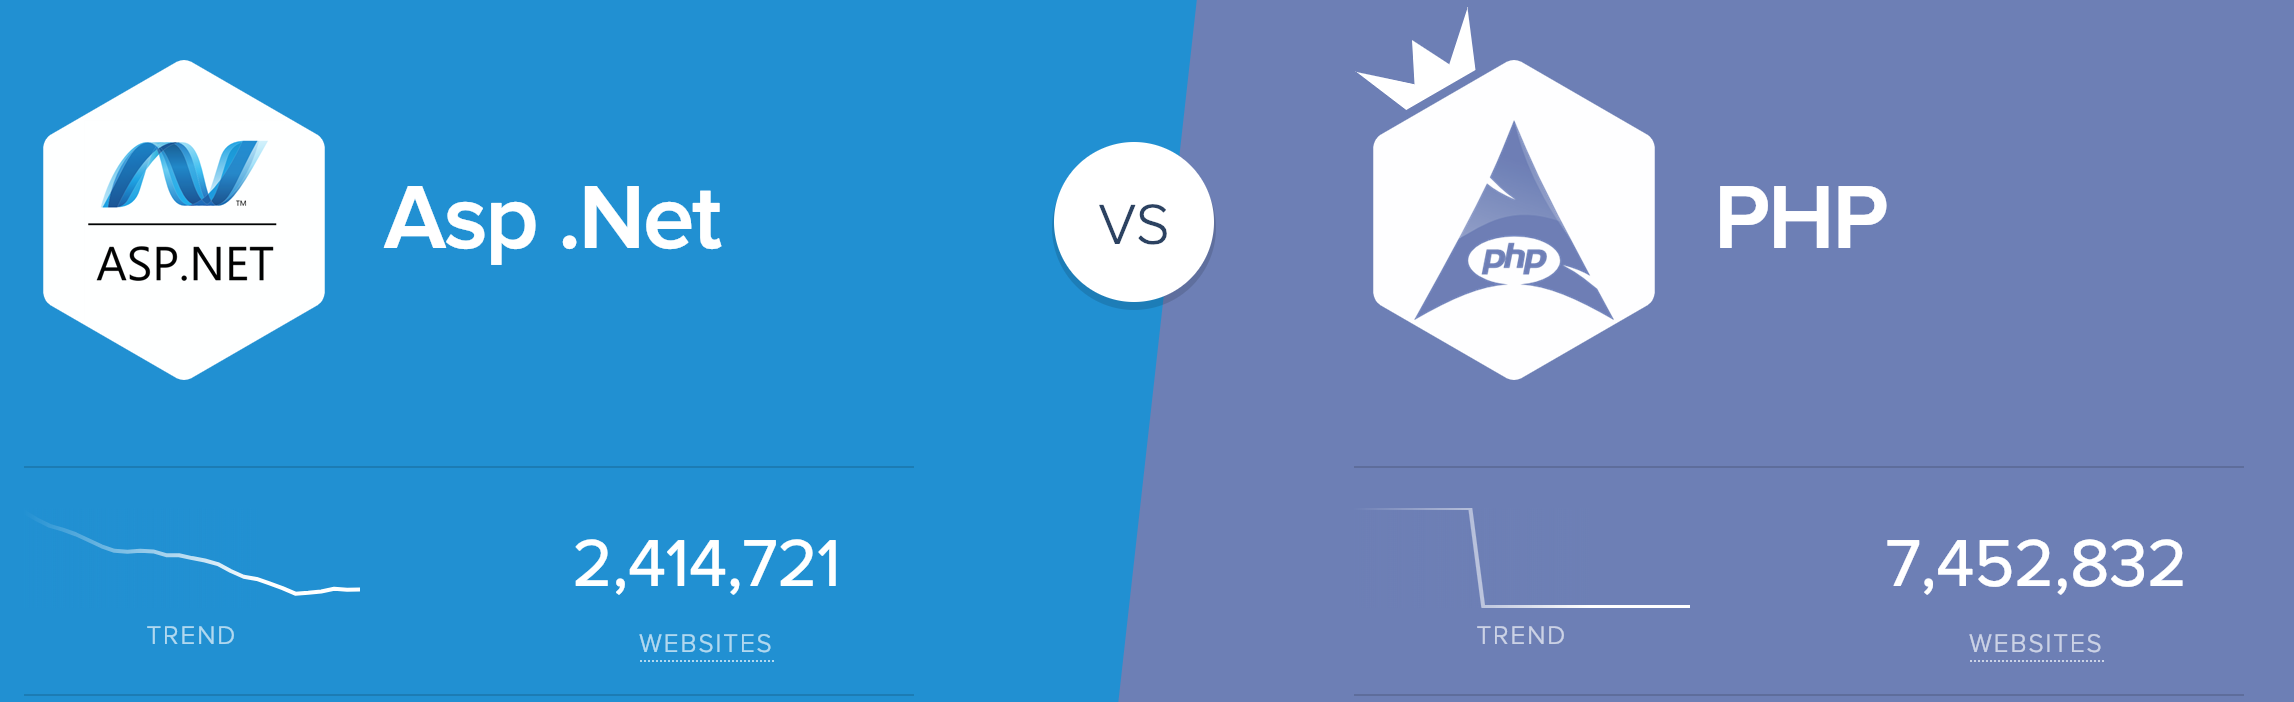
\includegraphics[scale = 0.3]{websites.png}
			\end{center}
			%the 
			\caption{Comparison of the technologies based on number of websites developed using them}
			\label{websites}
	\end{figure}

	\indent
	There has been found  a study~\citep{mirzoev2014webpage} that a compares the technologies by the webpage load spped. The authors created two small types of websites using both technologies: i) test.aspx \& test.php and ii) about.aspx \& about.php. The first type of website, \textit{test.*}, called 3 JavaScript files, 1 style sheet, 4 images and 1 favicon. The second type of website, \textit{about.*}, read a text file with 10.000 lines (each line being 15 characters long) and displayed it in the webpage. The webpage load speed was recorded using an addon, Lori (Life-of-request info), in Mozilla Firefox browser, the results can be seen in Figure~\ref{speedFig}. In both sessions PHP ran faster than ASP.NET (session 1 -> 0.189 s, session 2 -> 1.281), however, PHP also had one the slowest loading time in session 1 -> 0.304 seconds. In \textit{Session 1} ASP.NET average load time was faster with 11.2 miliseconds than PHP while in \textit{Session 2} PHP website loaded faster on average with 13.56 miliseconds than the one using in ASP.NET. It seems from this study that there is not a big difference between ASP.NET and PHP when it comes to webpage load speed. However, the author belives that a more thorough testing scenario could be designed in order to validate the results of the above mentioned study. 

\begin{figure}[H]

	\begin{center}
			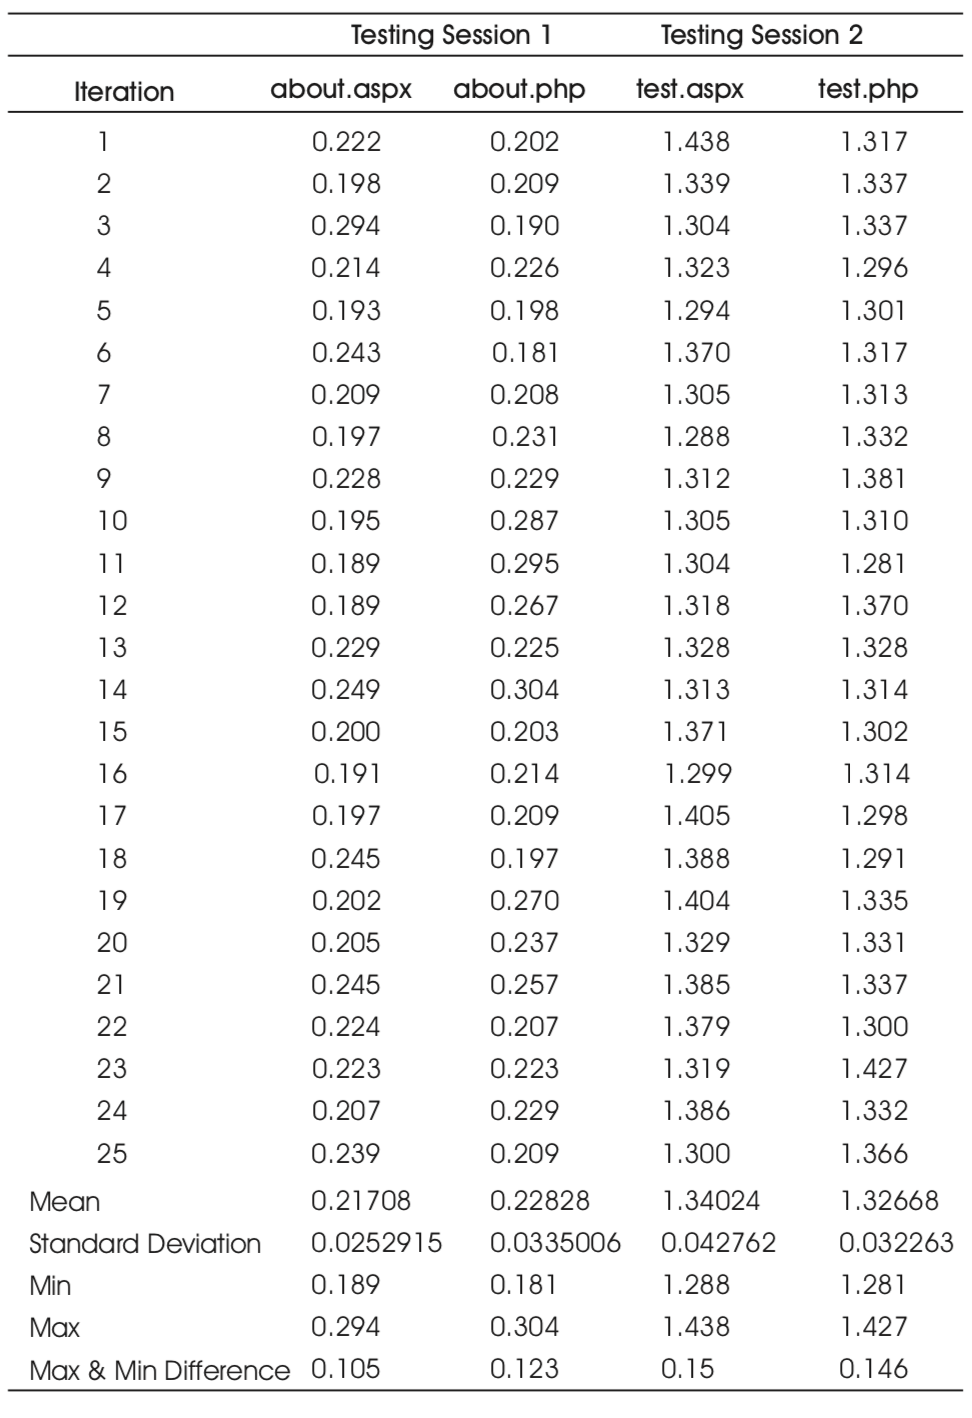
\includegraphics[scale = 0.5]{speedComp.png}
	\end{center}
	%the 
	\caption{Speed comparisons between two webpages written using both technologies}
	\label{speedFig}

\end{figure}

%Using php can sometime increase the dev time because of spending much time getting separate components written by other people work together whereas ASP.NET modules generally all work well together 

\section{Conclusion}(1000 words)
%Microsoft has made a big step by making ASP.NET open source and providing cross-platform development, over time this might increase the adoption of ASP.NET by the developer community.

\pagebreak

\bibliographystyle{agsm}
\bibliography{asp_net_vs_php}

\end{document}

